% !TeX spellcheck = en_GB
% !TeX program = pdflatex

\documentclass[10pt, a4paper]{article}

\usepackage[T1]{fontenc}
\usepackage[utf8]{inputenc}
\usepackage[british]{babel}
\usepackage[left=0mm,right=0mm,top=0mm,bottom=0mm]{geometry}
\usepackage[stretch=20,shrink=20,tracking=true,letterspace=25]{microtype}
\usepackage{graphicx}
\usepackage{xcolor}
\usepackage{marvosym}
\usepackage{fontawesome5}
\usepackage{enumitem}
\usepackage{FiraSans}
\usepackage[colorlinks=true,urlcolor=white,linkcolor=white]{hyperref}

\renewcommand{\familydefault}{\sfdefault}
\setlist{parsep=0pt,topsep=2pt,partopsep=0pt,itemsep=2pt,leftmargin=5mm}

\definecolor{cvblue}{HTML}{304263}

\newcommand{\dates}[1]{\textbf{#1}}
\newcommand{\is}{\par\vskip0.45ex}
\newcommand{\smaller}[1]{{\small$\diamond$\ #1}}
\newcommand{\headleft}[1]{\vspace*{2.2ex}\textsc{\textbf{#1}}\par\vspace*{-1.2ex}\hrulefill\par\vspace*{0.5ex}}
\newcommand{\headright}[1]{\vspace*{1.8ex}\textsc{\large\color{cvblue}#1}\par\vspace*{-1.5ex}{\color{cvblue}\hrulefill}\par\vspace*{0.3ex}}

\begin{document}
\setlength{\topskip}{0pt}
\setlength{\parindent}{0pt}
\setlength{\parskip}{0pt}
\setlength{\fboxsep}{0pt}
\pagestyle{empty}
\raggedbottom

\begin{minipage}[t]{0.33\textwidth}
\colorbox{cvblue}{\begin{minipage}[t][4mm][t]{\textwidth}\null\hfill\null\end{minipage}}

\vspace{-.2ex}
\colorbox{cvblue!92}{\color{white}
\kern0.08\textwidth
\begin{minipage}[t][293mm][t]{0.84\textwidth}
\raggedright
\vspace*{2.2ex}

{\Large Petr \textbf{\textsc{\v{S}im\v{c}\'ak}}} \normalsize

\null\hfill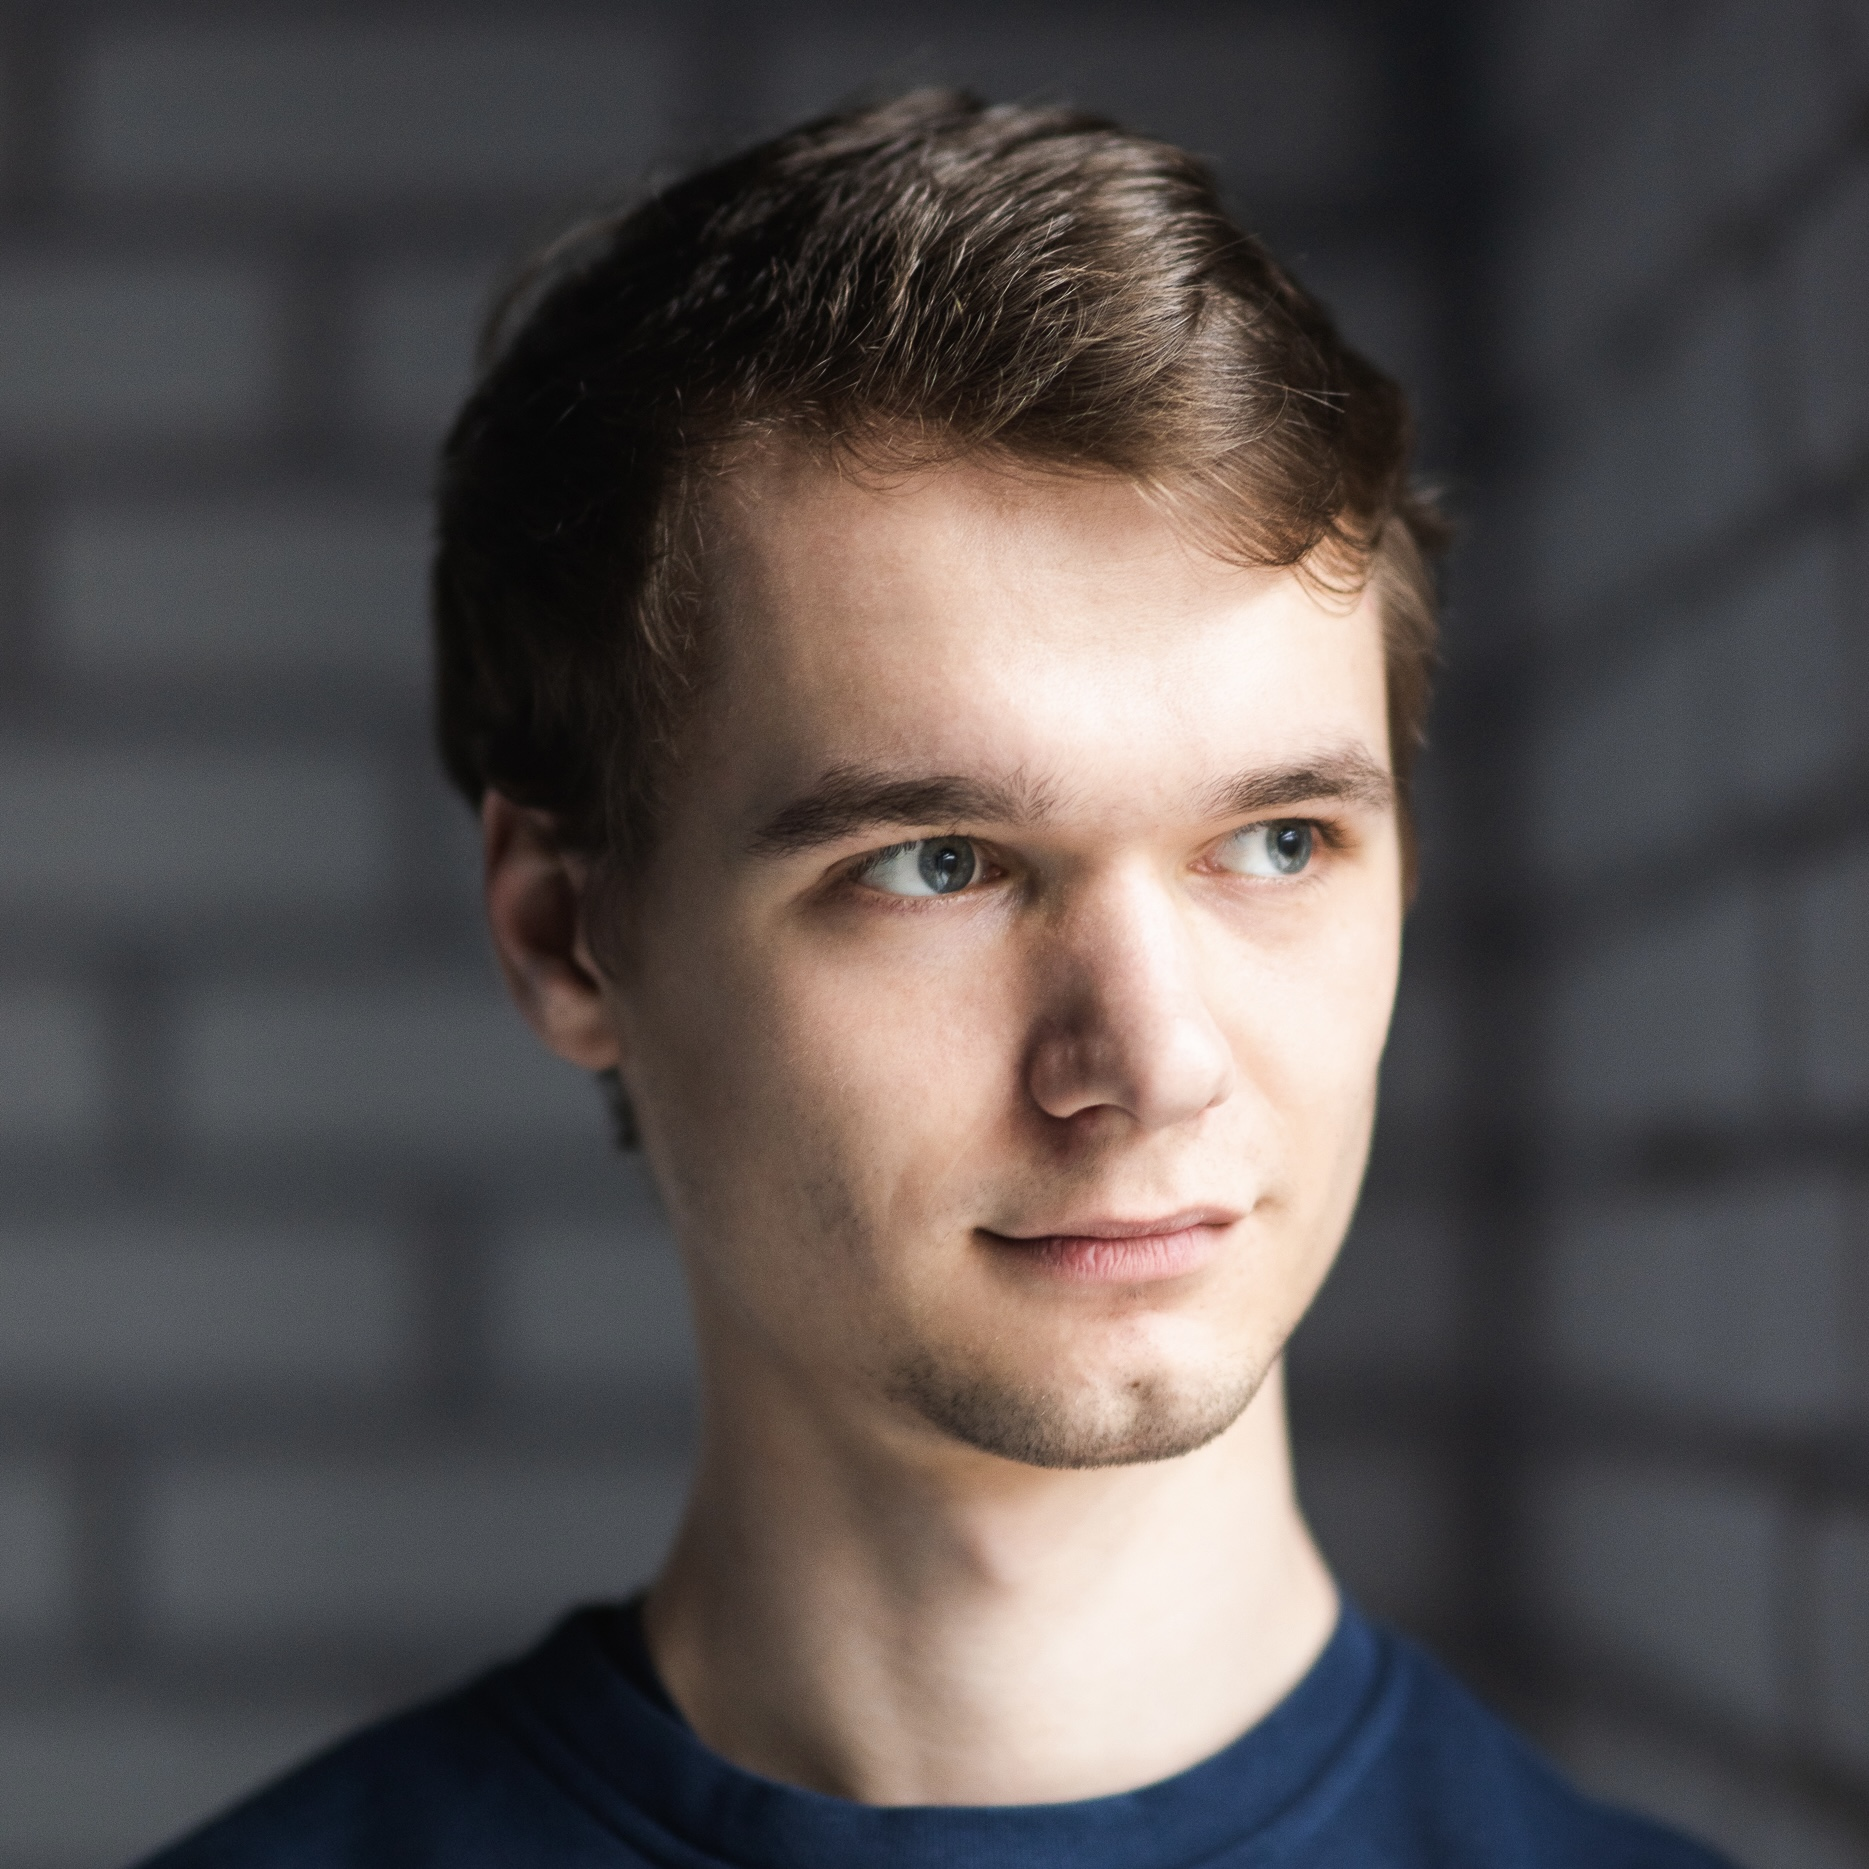
\includegraphics[width=0.62\textwidth]{me.jpg}\hfill\null

\vspace*{0.4ex}

\headleft{Profile}
Software developer with strong foundations in C, C++, and Python through 42 Prague and academic project work. Experience includes parsing, networking, Unix process handling, Docker-based environments, and signal-processing workflows.

\headleft{Contact}
\small
\MVAt\ \href{mailto:peta.simcak@gmail.com}{peta.simcak@gmail.com} \\[0.4ex]
\Mobilefone\ +420\,601\,381\,619 \\[0.4ex]
\Mundus\ \href{https://simcak.github.io}{simcak.github.io} \\[0.4ex]
\Letter\ Prague, Czech Republic \\[0.4ex]
\faGithub\ \href{https://github.com/simcak}{github.com/simcak} \\[0.4ex]
\faLinkedin\ \href{https://www.linkedin.com/in/petr-simcak}{linkedin.com/in/petr-simcak}
\normalsize

\headleft{Technical stack}
\begin{itemize}
\item C, C++, Python, Bash, MATLAB
\item Git, Docker, Linux, Nginx, LaTeX
\item Sockets, parsing, Unix processes
\item Backend workflows, signal processing
\end{itemize}

\headleft{Human languages}
Czech~(native) \\
English~(fluent) \\
German~(B1)

\headleft{Links}
\small
\href{https://github.com/simcak/Core/tree/main/11_CUB3D}{Cub3D repository} \\[0.3ex]
\href{https://github.com/simcak/Core/tree/main/14_IRC}{ft\_irc repository} \\[0.3ex]
\href{https://github.com/simcak/bakalarka}{Thesis repository}
\normalsize

\end{minipage}
\kern0.08\textwidth
}
\end{minipage}
\hskip2.2em
\begin{minipage}[t]{0.57\textwidth}
\setlength{\parskip}{0.55ex}

\vspace{1.5ex}

\headright{Technical projects}

\dates{2026--ongoing} \\
\textsc{ft\_transcendence} \textit{(full-stack web application)} \\
\smaller{Current team-based 42 project focused on a larger end-to-end application.}

\is
\dates{2026} \\
\textsc{ft\_irc} \textit{(C++98, non-blocking sockets, poll)} \\
\smaller{Built a minimal multi-client IRC server in a team of three; responsible for cleaning server-side code and implementing IRC commands.}

\is
\dates{2025} \\
\textsc{Cub3D} \textit{(C, MLX42, raycasting)} \\
\smaller{Implemented map parsing and core raycasting logic in a simplified Wolfenstein-style engine.}

\is
\dates{2025} \\
\textsc{Heart Rate Estimation from PPG Signals} \textit{(Python, signal processing)} \\
\smaller{Compared multiple HR-estimation methods, including a Hjorth descriptor-based approach, and worked on automatic PPG signal-quality classification.}

\is
\dates{2024--2025} \\
\textsc{Additional 42 projects} \textit{(C, Docker, Linux)} \\
\smaller{minishell: Unix processes, pipes, redirections. Inception: containerized multi-service setup with Docker and Nginx.}

\headright{Education}

\dates{2023--2026} \\
\textsc{42 Prague} \textit{(42 Heilbronn: 2024--2025)} \\
\smaller{Project-based software engineering curriculum with emphasis on low-level programming, problem solving, and peer learning.}

\is
\dates{2020--2025} \\
\textsc{Brno University of Technology} \\
\smaller{Bachelor's Degree in Sport Technology. Thesis: \textit{Heart Rate Estimation from the PPG Signals}.}

\headright{Additional experience}

\dates{2026--present} \\
\textsc{Tutor at 42 Prague} \\
\smaller{Support students with debugging, project understanding, and technical problem solving.}

\is
\dates{2025} \\
\textsc{\v{S}koda B3R Brigade} \textit{--- Team Lead / Backend Developer} \\
\smaller{2nd place at \v{S}koda Hackathon; backend work on a talent-matching application using FastAPI, React, Docker, and SQLite.}

\is
\dates{2022--present} \\
\textsc{3D Printer Maintenance and Support} \\
\smaller{Assembled a 3D printer at BUT and later maintained and supported it at 42 Prague.}

\is
\dates{2013--2021} \\
\textsc{Film / theatre background} \\
\smaller{Earlier professional experience in collaborative performance environments; developed communication, discipline, and adaptability.}

\end{minipage}

\end{document}